\documentclass[journal,12pt,twocolumn]{IEEEtran}
%
\usepackage{setspace}
\usepackage{gensymb}
%\doublespacing
\singlespacing

%\usepackage{graphicx}
%\usepackage{amssymb}
%\usepackage{relsize}
\usepackage[cmex10]{amsmath}
%\usepackage{amsthm}
%\interdisplaylinepenalty=2500
%\savesymbol{iint}
%\usepackage{txfonts}
%\restoresymbol{TXF}{iint}
%\usepackage{wasysym}
\usepackage{amsthm}
%\usepackage{iithtlc}
\usepackage{mathrsfs}
\usepackage{txfonts}
\usepackage{stfloats}
\usepackage{bm}
\usepackage{cite}
\usepackage{cases}
\usepackage{subfig}
%\usepackage{xtab}
\usepackage{longtable}
\usepackage{multirow}
\usepackage{algorithm}
\usepackage{algpseudocode}
\usepackage{enumitem}
\usepackage{mathtools}
\usepackage{tikz}
\usepackage{circuitikz}
\usepackage{verbatim}
%\usepackage{tfrupee}
\usepackage[breaklinks=true]{hyperref}
%\usepackage{stmaryrd}
\usepackage{tkz-euclide} % loads  TikZ and tkz-base
%\usetkzobj{all}
\usepackage{listings}
    \usepackage{color}                                            %%
    \usepackage{array}                                            %%
    \usepackage{longtable}                                        %%
    \usepackage{calc}                                             %%
    \usepackage{multirow}                                         %%
    \usepackage{hhline}                                           %%
    \usepackage{ifthen}                                           %%
  %optionally (for landscape tables embedded in another document): %%
    \usepackage{lscape}     
\usepackage{multicol}
\usepackage{chngcntr}
%\usepackage{enumerate}
\usepackage{karnaugh-map}

%\usepackage{wasysym}
%\newcounter{MYtempeqncnt}
\DeclareMathOperator*{\Res}{Res}
%\renewcommand{\baselinestretch}{2}
\renewcommand\thesection{\arabic{section}}
\renewcommand\thesubsection{\thesection.\arabic{subsection}}
\renewcommand\thesubsubsection{\thesubsection.\arabic{subsubsection}}

\renewcommand\thesectiondis{\arabic{section}}
\renewcommand\thesubsectiondis{\thesectiondis.\arabic{subsection}}
\renewcommand\thesubsubsectiondis{\thesubsectiondis.\arabic{subsubsection}}

% correct bad hyphenation here
\hyphenation{op-tical net-works semi-conduc-tor}
\def\inputGnumericTable{}                                 %%

\lstset{
%language=C,
frame=single, 
breaklines=true,
columns=fullflexible
}
%\lstset{
%language=tex,
%frame=single, 
%breaklines=true
%}

\begin{document}
%


\newtheorem{theorem}{Theorem}[section]
\newtheorem{problem}{Problem}
\newtheorem{proposition}{Proposition}[section]
\newtheorem{lemma}{Lemma}[section]
\newtheorem{corollary}[theorem]{Corollary}
\newtheorem{example}{Example}[section]
\newtheorem{definition}[problem]{Definition}
%\newtheorem{thm}{Theorem}[section] 
%\newtheorem{defn}[thm]{Definition}
%\newtheorem{algorithm}{Algorithm}[section]
%\newtheorem{cor}{Corollary}
\newcommand{\BEQA}{\begin{eqnarray}}
\newcommand{\EEQA}{\end{eqnarray}}
\newcommand{\define}{\stackrel{\triangle}{=}}
\bibliographystyle{IEEEtran}
%\bibliographystyle{ieeetr}
\providecommand{\mbf}{\mathbf}
\providecommand{\pr}[1]{\ensuremath{\Pr\left(#1\right)}}
\providecommand{\qfunc}[1]{\ensuremath{Q\left(#1\right)}}
\providecommand{\sbrak}[1]{\ensuremath{{}\left[#1\right]}}
\providecommand{\lsbrak}[1]{\ensuremath{{}\left[#1\right.}}
\providecommand{\rsbrak}[1]{\ensuremath{{}\left.#1\right]}}
\providecommand{\brak}[1]{\ensuremath{\left(#1\right)}}
\providecommand{\lbrak}[1]{\ensuremath{\left(#1\right.}}
\providecommand{\rbrak}[1]{\ensuremath{\left.#1\right)}}
\providecommand{\cbrak}[1]{\ensuremath{\left\{#1\right\}}}
\providecommand{\lcbrak}[1]{\ensuremath{\left\{#1\right.}}
\providecommand{\rcbrak}[1]{\ensuremath{\left.#1\right\}}}
\theoremstyle{remark}
\newtheorem{rem}{Remark}
\newcommand{\sgn}{\mathop{\mathrm{sgn}}}
\providecommand{\abs}[1]{$\left\vert#1\right\vert$}
\providecommand{\res}[1]{\Res\displaylimits_{#1}} 
\providecommand{\norm}[1]{$\left\lVert#1\right\rVert$}
%\providecommand{\norm}[1]{\lVert#1\rVert}
\providecommand{\mtx}[1]{\mathbf{#1}}
\providecommand{\mean}[1]{E$\left[ #1 \right]$}
\providecommand{\fourier}{\overset{\mathcal{F}}{ \rightleftharpoons}}
%\providecommand{\hilbert}{\overset{\mathcal{H}}{ \rightleftharpoons}}
\providecommand{\system}{\overset{\mathcal{H}}{ \longleftrightarrow}}
	%\newcommand{\solution}[2]{\textbf{Solution:}{#1}}
\newcommand{\solution}{\noindent \textbf{Solution: }}
\newcommand{\cosec}{\,\text{cosec}\,}
\providecommand{\dec}[2]{\ensuremath{\overset{#1}{\underset{#2}{\gtrless}}}}
\newcommand{\myvec}[1]{\ensuremath{\begin{pmatrix}#1\end{pmatrix}}}
\newcommand{\mydet}[1]{\ensuremath{\begin{vmatrix}#1\end{vmatrix}}}
\makeatletter
\@addtoreset{figure}{problem}
\makeatother
\let\StandardTheFigure\thefigure
\let\vec\mathbf
%\renewcommand{\thefigure}{\theproblem.\arabic{figure}}
\renewcommand{\thefigure}{\theproblem}
%\setlist[enumerate,1]{before=\renewcommand\theequation{\theenumi.\arabic{equation}}
%\counterwithin{equation}{enumi}
%\renewcommand{\theequation}{\arabic{subsection}.\arabic{equation}}
\def\putbox#1#2#3{\makebox[0in][l]{\makebox[#1][l]{}\raisebox{\baselineskip}[0in][0in]{\raisebox{#2}[0in][0in]{#3}}}}
     \def\rightbox#1{\makebox[0in][r]{#1}}
     \def\centbox#1{\makebox[0in]{#1}}
     \def\topbox#1{\raisebox{-\baselineskip}[0in][0in]{#1}}
     \def\midbox#1{\raisebox{-0.5\baselineskip}[0in][0in]{#1}}
\vspace{3cm}
\title{
%	\logo{
EE 5811 : FPGA LAB \\ Challenge Problem 2
%	}
}
\author{ Shantanu Yadav (EE20MTECH12001)}	
% make the title area
\maketitle
\newpage
%\tableofcontents
\bigskip
\renewcommand{\thefigure}{\theenumi}
\renewcommand{\thetable}{\theenumi}
%\renewcommand{\theequation}{\theenumi}
Download the codes from
\begin{lstlisting}
https://github.com/Shantanu2508/mtech/tree/master/FPGA_LAB/CP2
\end{lstlisting}

\section{PROBLEM STATEMENT}
Is it possible to implement the NAND logic using some data structure/algorithm?

\section{THEORY}
A NAND (NOT-AND) gate produces a False output only if all the inputs are True. The truth table is as follows
\begin{table}[h]
    \centering
    \begin{tabular}{|c|c|c|c|}
    \hline
    $X$&$Y$&OUT  \\
    \hline
    0&0&1\\
    0&1&1\\
    1&0&1\\
    1&1&0\\
    \hline
    \end{tabular}
    \caption{Truth table for NAND gate}
\end{table}
The NAND gate is a universal gate because any boolean function can be implemented by using a combination of NAND gates. One interesting property of NAND logic is that if any of the input is LOW the corresponding output is HIGH. This logic can be realised using stack data structure. Stacks are abstract data structures based on LIFO (Last In First Out) technique. The two main principal operations are push and pop. Push operation adds an element to the stack and pop operation removes an element from the top of the stack. \\

To implement NAND logic we first create an empty stack. The input to the NAND gate is assumed to be an array of size $N \times 2$, where $N$ are the total number of input combinations. For each input stream, $X$ is pushed into the stack and compared with $Y$. If any of them is 0 the output is 1 otherwise if the top element of stack and the Y input are both equal to 1 then output is false. 

\begin{algorithm}
\caption{NAND Logic using stack data structure }\label{alg:cap}
\begin{algorithmic}
\Require Array of size $N \times 2$
\Ensure Create an empty stack $S$
\State $i \gets 0$
\While{$i \leq N-1$}
\State $S \gets input[i][0]$
\If{$S.top() == 0$}
    \State $output[i] \gets 1$
    \State $i \gets i+1$
\ElsIf{$input[i][1] == 0$}
    \State $output[i] \gets 1$
    \State $i \gets i+1$
\Else{}
    \State $output[i] \gets 0$
    \State $i \gets i+1$
\EndIf
\State $S.pop()$

\EndWhile
\end{algorithmic}
\end{algorithm}

\section{EXAMPLE}
Implement the boolean expresion given below using NAND gates
\begin{align}
    F(X,Y) = X + \Bar{Y} 
\end{align}
The logic circuit is realised using NAND gates as in shown figure below \\

 \\ 
 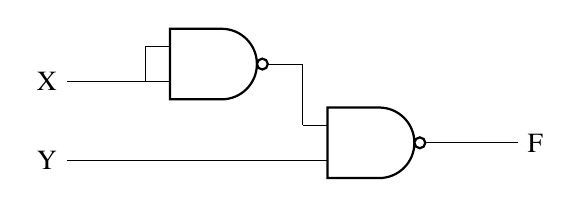
\begin{tikzpicture}
% Circuit style
\ctikzset{
    logic ports=ieee,
logic ports/scale=0.8
}
% Logic ports
\node[nand port] (na) at (0,1){};
\node[nand port] (nb) at (2,0){};
\draw (na.out) -| (nb.in 1);
\draw (na.in 2) -| (na.in 1);
\draw (nb.in 2) -| ++(-3,0)node[left](Y){Y};
\draw (na.in 2) -| ++(-1,0)node[left](X){X};
\draw (nb.out) -| ++(1,0)node[right](F){F};
\end{tikzpicture}

\begin{table}[h]
    \centering
    \begin{tabular}{|c|c|c|}
    \hline
    $X$&$Y$&F  \\
    \hline
    0&0&1\\
    0&1&0\\
    1&0&1\\
    1&1&1\\
    \hline
    \end{tabular}
    \caption{Truth Table for $F = X + \Bar{Y}$. (Verified using code)}
\end{table}
\\
If ${X}$ and ${Y}$ are sets containing only 0 and 1 then the input stream to the NAND logic can be defined as,
\begin{align}
    S = \left\{ \ (x,y) \ | \  x \in X, \  y\in Y \ \right \}
\end{align}
where each $(x,y)$ pair is an input to the NAND gate at any time instant.
The NAND logic can be interpreted as a function $g:S \rightarrow \{0,1\}$ defined as,
\begin{align}
 g(x,y) = 
 \begin{cases}
 0, & x = 1  \  \text{and} \ y = 1 \\
 1, & \text{otherwise}
 \end{cases}
\end{align}
 Thus from the above figure, the boolean expression can be expressed as
\begin{align}
    F = g(g(x,x),y)
\end{align}
Each time when function $g$ is invoked, the $x$ value of the first input is pushed into the stack. If $x = 0$ the output is 1 regardless of $y$, but if $x = 1$ the output is 1 if $y = 0$ otherwise the output is 0. After this $x$ is removed from the stack and the procedure repeats for other inputs.
\end{document}